\section{実験}
\subsection{実験条件}
COCO 2017 Validationの5000枚を重複しない検証用とテスト用に分割する．
検証用はseed 42でサンプリングした500枚（dev500）とLVIS\cite{ref_LVIS}のアノテーションが存在する2604枚（lvis\_dev）であり，テスト用は残りの画像から別にサンプリングした500枚（test500，GTインスタンス3748件）とLVISのアノテーションが存在する2148枚（lvis\_test）である．
本稿の結果はすべてテスト用の分割の値であり，$ \tau $はlvis\_devで階層的F値$ hF $が最大となる値を選んだ．
検出スコアの閾値は，評価インスタンス数が近い組である，DETRの$ \theta = 0.5 $（以下，proposed）とYOLO11xの0.25（以下，hybrid）を主に示す．
COCOのGTとIoUが0.5以上で対応した検出について，深さ0のTop-1正解率を評価する．
深さ1以降は，COCOのカテゴリより細かいLVISのSynsetをIoUが0.5以上で対応付けたインスタンス（proposedで489件，hybridで481件）について，COCOのSynsetからLVISのSynsetまでの経路を正解とする階層的適合率$ hP $，再現率$ hR $，F値$ hF $\cite{ref_hF}で評価する．
COCO外の物体の評価には，lvis\_testにおいて，SynsetがCOCOのカテゴリの上位語・下位語でなく，レンマ名もCOCOのカテゴリ名と一致しないLVISのアノテーション（511カテゴリ）に対応し，COCOのGTとは対応しない検出ボックスを用いる．
評価インスタンスはhybridで262件（117カテゴリ），proposedで521件（175カテゴリ）である．
深さ0の語がLVISのSynsetの上位語または自身である割合を，COCO外の物体の正解率とする．

\subsection{ソフトマックスとシグモイドの比較}
表\ref{tab_normalization}と図\ref{fig_auroc}にVLMと正規化関数ごとの結果を示す．
図\ref{fig_auroc}(a)は，test500において深さ0が正しい枝と誤った枝を，最深段の確信度で区別する性能をAUROCで示す．
図\ref{fig_auroc}(b)は，lvis\_testにおいて深さ0が正しいインスタンスの深さ1の正誤を，深さ1の確信度で区別する性能をAUROCで示す．

\begin{table*}[t]
    \centering
    \caption{VLMと正規化関数の比較（テスト用の分割）．Top-1はtest500の深さ0のTop-1正解率，誤枝AUROCは深さ0の正誤を最深段の確信度および累積確信度で区別するAUROC，深さ1はlvis\_testで深さ0が正しいインスタンスの深さ1の正解率と，深さ1の確信度による正誤のAUROC，$ hF $は$ \tau $による停止規則と深さの上限1による停止規則のlvis\_testの階層的F値である．}
    \label{tab_normalization}
    \begin{tabular}{llcccccccc}
        \toprule
        & & & \multicolumn{2}{c}{誤枝AUROC} & \multicolumn{2}{c}{深さ1} & \multicolumn{3}{c}{$ hF $} \\
        \cmidrule(lr){4-5} \cmidrule(lr){6-7} \cmidrule(lr){8-10}
        手法 & VLMと正規化関数 & Top-1 & 最深段 & 累積 & 正解率 & AUROC & $ \tau $ & $ \tau $による停止 & 深さ1まで \\
        \midrule
        \multirow{3}{*}{proposed} & CLIP + ソフトマックス & 0.552 & 0.611 & 0.508 & 0.440 & 0.744 & 0.2 & 0.462 & 0.451 \\
        & SigLIP + ソフトマックス & 0.527 & 0.600 & 0.634 & 0.462 & 0.843 & 0.5 & 0.480 & 0.453 \\
        & SigLIP + シグモイド & 0.527 & 0.715 & 0.633 & 0.462 & 0.587 & $ 10^{-4} $ & 0.450 & 0.453 \\
        \midrule
        \multirow{3}{*}{hybrid} & CLIP + ソフトマックス & 0.969 & 0.418 & 0.430 & 0.407 & 0.762 & 0.3 & 0.647 & 0.648 \\
        & SigLIP + ソフトマックス & 0.969 & 0.480 & 0.483 & 0.405 & 0.780 & 0.3 & 0.648 & 0.648 \\
        & SigLIP + シグモイド & 0.969 & 0.617 & 0.594 & 0.405 & 0.644 & 0.05 & 0.659 & 0.648 \\
        \bottomrule
    \end{tabular}
\end{table*}

\begin{figure}[t]
    \centering
    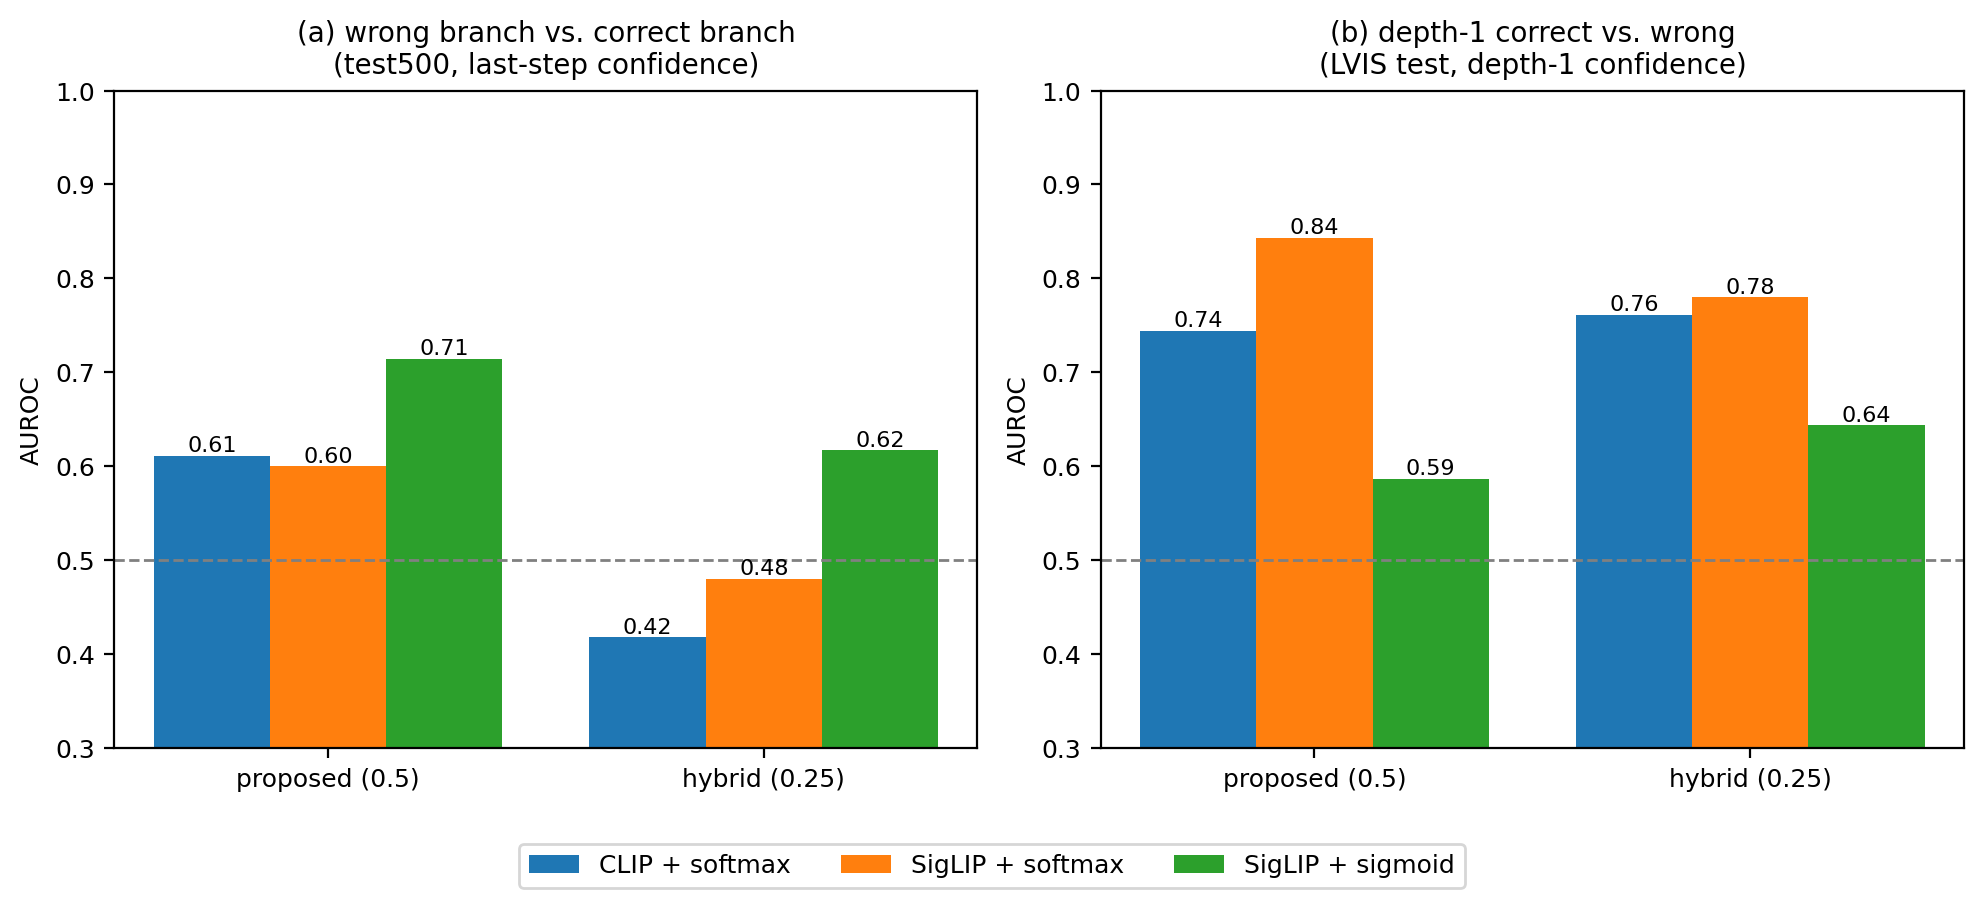
\includegraphics[width=\linewidth]{figures/fig_auroc.png}
    \caption{確信度による正誤の識別性能．(a)はtest500で深さ0が正しい枝と誤った枝を最深段の確信度で区別するAUROC，(b)はlvis\_testで深さ0が正しいインスタンスの深さ1の正誤を深さ1の確信度で区別するAUROCである．破線は偶然の水準0.5である．}
    \label{fig_auroc}
\end{figure}

表\ref{tab_normalization}から，SigLIPのTop-1正解率はproposedでCLIPより0.025低く，hybridでは深さ0がYOLOで決まるため同じである．
図\ref{fig_auroc}(a)から，シグモイドは誤った枝の識別性能を，hybridで0.418から0.617へ，proposedで0.611から0.715へ改善した．
SigLIPにソフトマックスを用いた場合のhybridのAUROCは0.480であり，この改善はモデルの変更ではなく正規化関数の変更によるものである．
ソフトマックスでは，誤った枝の候補語彙に正しい語が含まれなくても候補の中で相対的に最もよい語の確信度が高くなるのに対し，シグモイドでは画像と語の対応が弱い場合に確信度が低くなるためである．
一方，図\ref{fig_auroc}(b)から，深さ0が正しい場合の深さ1の正誤の識別では，ソフトマックスがシグモイドより高いAUROCを示した．
SigLIPでは，ソフトマックスの0.843（proposed）および0.780（hybrid）に対し，シグモイドは0.587および0.644であった．
兄弟の語の中での相対的な比較が必要な深さ1の判断では，候補語彙の中で正規化するソフトマックスが有利である．

図\ref{fig_stopping_scorers}にlvis\_testにおける停止規則の$ hP $と$ hR $の関係を示す．
横軸は階層的再現率$ hR $，縦軸は階層的適合率$ hP $であり，曲線は$ \tau $を変化させた累積確信度による停止規則，四角は深さの上限（0〜3）による停止規則である．
hybridでは，シグモイドの$ \tau = 0.05 $による停止が$ hF = 0.659 $となり，CLIPとソフトマックスの0.647および深さの上限1の0.648をわずかに上回った．
proposedでは，シグモイドの深さ0の確信度が小さいため，$ \tau $を大きくすると多くのインスタンスが深さ0で棄却され，$ hP $の高い領域で他の組より劣った．
シグモイドの深い段階の確信度は0.01以下となる場合が多く，選ばれた$ \tau $は$ 10^{-4} $および0.05と小さい値であった．

\begin{figure}[t]
    \centering
    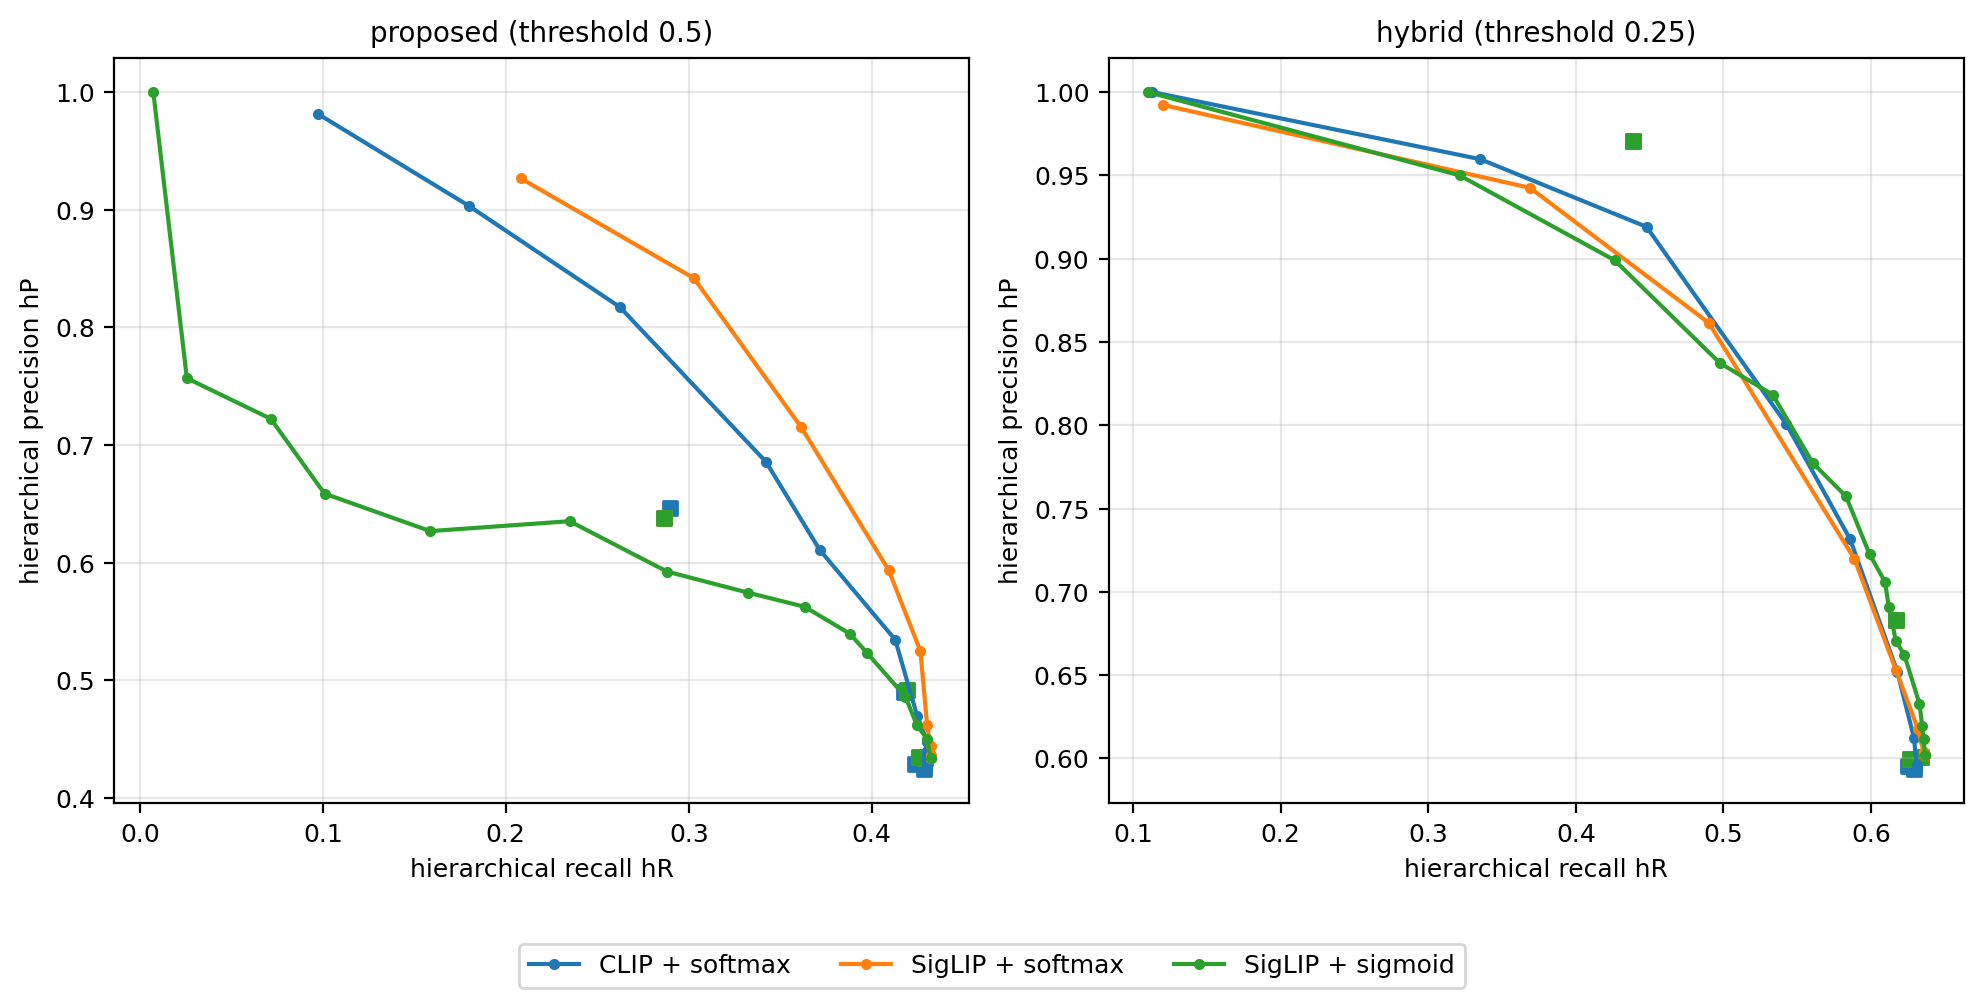
\includegraphics[width=\linewidth]{figures/fig_stopping_scorers.png}
    \caption{lvis\_testにおける階層的再現率$ hR $（横軸）と階層的適合率$ hP $（縦軸）の関係．曲線は累積確信度による停止規則，四角は深さの上限（0〜3）による停止規則である．}
    \label{fig_stopping_scorers}
\end{figure}

\subsection{YOLOとVLMのスコアの比較}
表\ref{tab_cmp}に，(\ref{eq_cmp})によるhybrid\_cmpのtest500の結果を示す．
切替はYOLOと異なる語が深さ0となったインスタンス数，改善と悪化はそれぞれYOLOの語が不正解でVLMの語が正解の数と，YOLOの語が正解でVLMの語が不正解の数である．

\begin{table}[t]
    \centering
    \caption{YOLOとVLMのスコアの比較による深さ0の決定（test500）．閾値はYOLO11xの検出スコアの閾値，Top-1の基準はYOLOの語をそのまま用いる場合のTop-1正解率である．}
    \label{tab_cmp}
    \small
    \setlength{\tabcolsep}{2.5pt}
    \begin{tabular}{clcccc}
        \toprule
        閾値 & VLMと正規化関数 & 切替 & 改善 & 悪化 & Top-1 \\
        \midrule
        \multirow{4}{*}{0.25} & 基準（hybrid） & -- & -- & -- & 0.969 \\
        & CLIP + ソフトマックス & 103 & 7 & 92 & 0.936 \\
        & SigLIP + ソフトマックス & 331 & 20 & 304 & 0.858 \\
        & SigLIP + シグモイド & 6 & 1 & 5 & 0.967 \\
        \midrule
        \multirow{4}{*}{0.7} & 基準（hybrid） & -- & -- & -- & 0.982 \\
        & CLIP + ソフトマックス & 21 & 0 & 21 & 0.969 \\
        & SigLIP + ソフトマックス & 127 & 5 & 122 & 0.908 \\
        & SigLIP + シグモイド & 1 & 0 & 1 & 0.982 \\
        \bottomrule
    \end{tabular}
\end{table}

表\ref{tab_cmp}から，ソフトマックスでは切替の大部分がYOLOの正解を不正解に変えており，Top-1正解率はCLIPで0.969から0.936へ，SigLIPで0.858へ低下した．
閾値0.25において，YOLOの検出スコアの中央値は0.787であるのに対し，VLMの最大確信度の中央値はCLIPとソフトマックスで0.391，SigLIPとソフトマックスで0.755，SigLIPとシグモイドで0.022であった．
VLMの最大確信度がYOLOの検出スコアを上回るインスタンスの割合は，それぞれ24.0\%，52.2\%，3.0\%であり，SigLIPとソフトマックスで切替が最も多い．
シグモイドではVLMの確信度がYOLOの検出スコアを上回ることがほとんどなく，切替は6件にとどまり，Top-1正解率はほぼ変わらなかった．
YOLOの検出スコアとVLMの確信度は異なるモデルの異なる尺度の値であり，(\ref{eq_cmp})の切替の頻度は，予測の正しさではなく両者の尺度の違いで決まる．
なお，$ {\mathbb V}_0 $がCOCOの80クラスであるhybrid\_cmpは，COCO外の物体に正しい上位語を与えることはできず，COCO外の物体の正解率はすべての組で0であった．

\subsection{WordNetの同じ深さの語彙}
表\ref{tab_wn_vocab}に(\ref{eq_wn_vocab})の語彙の統計を示す．
COCO外の22語のうち語彙に含まれるのは，$ k = 2 $でmonkey，deer，fox，squirrelの4語であった．
penguin，camel，kangaroo，helicopter等は，COCOのカテゴリのいとこより深い語であるため含まれない．
lvis\_testのCOCO外の511カテゴリのうち，語彙に上位語または自身を持つカテゴリは$ k = 2 $で232カテゴリ（45\%）である．

\begin{table}[t]
    \centering
    \caption{WordNetの同じ深さの語彙の統計．COCO外はCOCOの80クラス以外の語数，22語はCOCO外の22語のうち語彙に含まれる語数，LVISはlvis\_testのCOCO外の511カテゴリのうち語彙に上位語または自身を持つカテゴリ数である．}
    \label{tab_wn_vocab}
    \begin{tabular}{ccccc}
        \toprule
        $ k $ & 語彙数 & COCO外 & 22語 & LVIS \\
        \midrule
        1 & 213 & 133 & 2 & 96 \\
        2 & 681 & 601 & 4 & 232 \\
        3 & 1115 & 1035 & 5 & 289 \\
        \bottomrule
    \end{tabular}
\end{table}

図\ref{fig_tradeoff}に，深さ0の決め方ごとの，COCOのTop-1正解率とCOCO外の物体の正解率の関係を示す．
横軸はtest500の深さ0のTop-1正解率，縦軸はlvis\_testのCOCO外の物体のうち深さ0の語がLVISのSynsetの上位語または自身である割合であり，閾値はいずれも0.25である．

\begin{figure}[t]
    \centering
    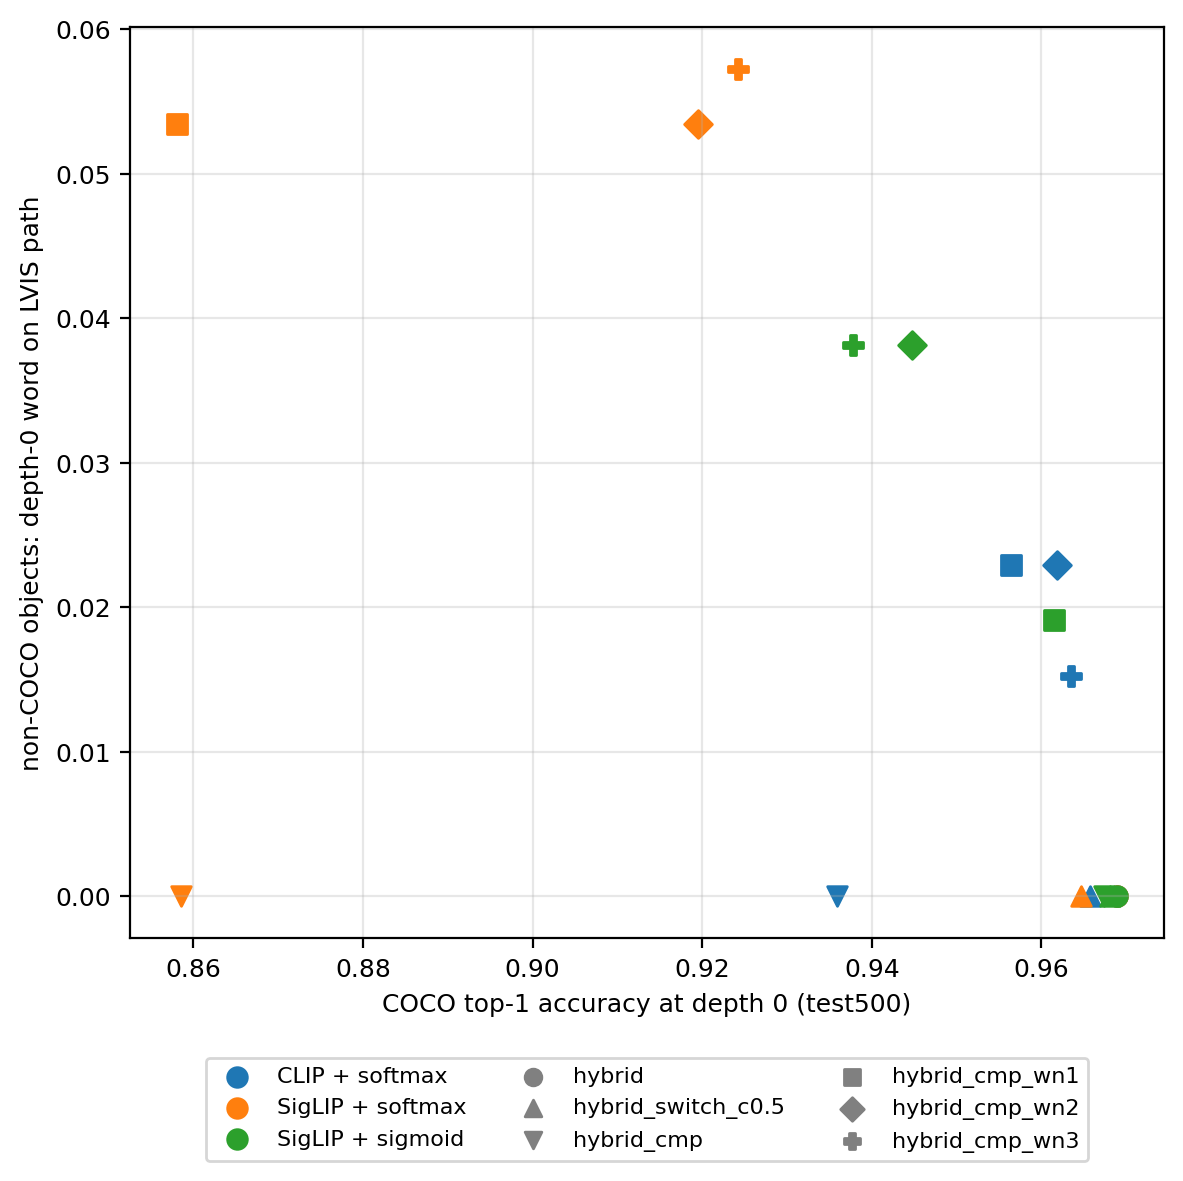
\includegraphics[width=0.9\linewidth]{figures/fig_tradeoff.png}
    \caption{COCOのTop-1正解率（横軸，test500）とCOCO外の物体の深さ0の正解率（縦軸，lvis\_test）の関係．色はVLMと正規化関数，形は深さ0の決め方を表し，YOLO11xの閾値は0.25である．}
    \label{fig_tradeoff}
\end{figure}

図\ref{fig_tradeoff}から，hybrid，hybrid\_switch\_c0.5およびhybrid\_cmpはCOCO外の物体の正解率が0である．
WordNetの同じ深さの語彙を用いたhybrid\_cmp\_wn2では，SigLIPとシグモイドでCOCO外の物体の正解率が3.8\%（262件中10件）に上がった一方，COCOのTop-1正解率は0.969から0.945へ低下した．
test500では65件がYOLOと異なる語に切り替わり，そのうち62件がYOLOの正解を不正解に変えた．
悪化の例は，personをleg，tvをscreen，ovenをstoveとするものであり，物体の部分や類義の語が選ばれている．
COCO外の物体で正しく命名できた例は，plate，can，pear，sack，pot，bucket等の容器や食品であった．
DETRに対して$ {\mathbb V}_0^{(2)} $から深さ0を選ぶproposed\_wn2では，COCO外の物体の正解率は10.0\%（SigLIP）であるが，COCOのTop-1正解率は0.527から0.304へ大きく低下した．
また，語彙には「slit」「worsted」「column」のように物体の名前として用いられにくい多義の語が含まれ，COCO外の物体の深さ0の上位にこれらの語が現れた．

図\ref{fig_qualitative}に，COCO外の物体の実画像に対する，SigLIPとシグモイドでの定性結果を示す．
上段の現在の構成（hybrid\_switch\_c0.5）では，penguinの3領域のうち2領域とcamelがCOCO外の語に切り替わった．
下段のhybrid\_cmp\_wn2では，penguinはbirdとなり，COCOと同じ深さの語としては正しい．
しかし，camelとkangarooは語彙に含まれないため，YOLOのdogとsheepのままであった．

\begin{figure*}[t]
    \centering
    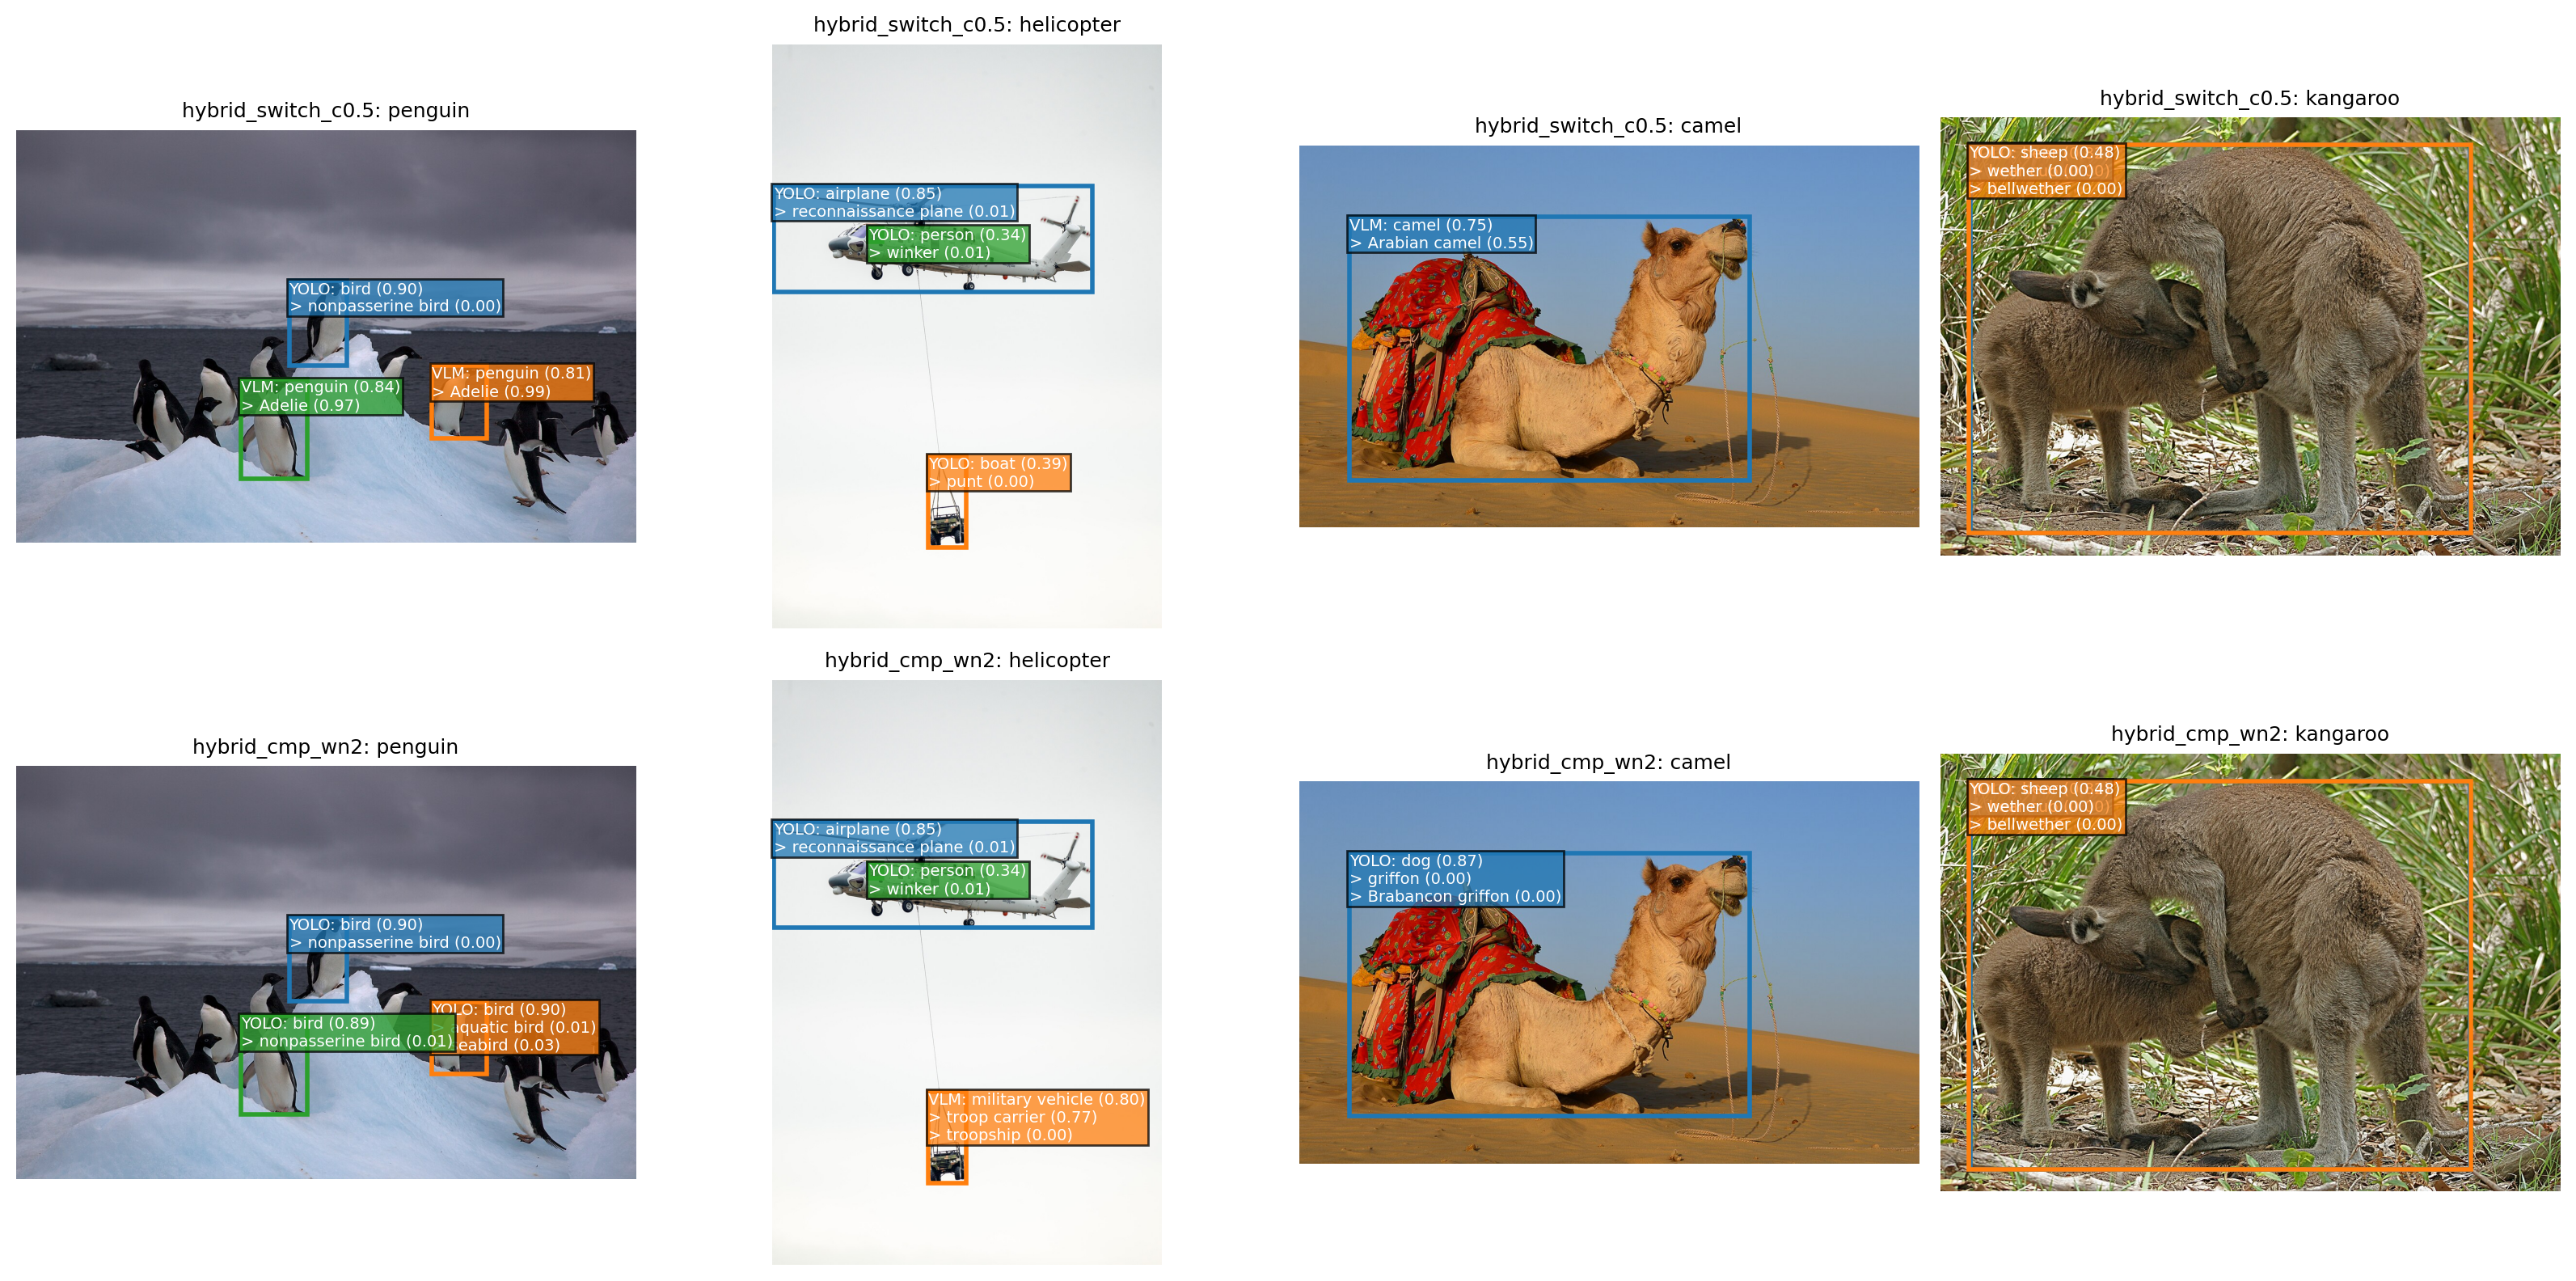
\includegraphics[width=0.85\linewidth]{figures/fig_qualitative.png}
    \caption{COCO外の物体の実画像に対する定性結果（SigLIPとシグモイド，YOLO11xの閾値0.25）．上段はCOCO外の22語への切替（hybrid\_switch\_c0.5），下段はWordNetの同じ深さの語彙とスコアの比較（hybrid\_cmp\_wn2）である．深さ0の語の前に，その決定に用いたモデルを``YOLO:''，``VLM:''で示す．画像はWikimedia Commons（CC BY 2.0，CC0，CC BY-SA 3.0/4.0）より取得した．}
    \label{fig_qualitative}
\end{figure*}
